
%% bare_conf.tex
%% V1.4b
%% 2015/08/26
%% by Michael Shell
%% See:
%% http://www.michaelshell.org/
%% for current contact information.
%%
%% This is a skeleton file demonstrating the use of IEEEtran.cls
%% (requires IEEEtran.cls version 1.8b or later) with an IEEE
%% conference paper.
%%
%% Support sites:
%% http://www.michaelshell.org/tex/ieeetran/
%% http://www.ctan.org/pkg/ieeetran
%% and
%% http://www.ieee.org/

%%*************************************************************************
%% Legal Notice:
%% This code is offered as-is without any warranty either expressed or
%% implied; without even the implied warranty of MERCHANTABILITY or
%% FITNESS FOR A PARTICULAR PURPOSE! 
%% User assumes all risk.
%% In no event shall the IEEE or any contributor to this code be liable for
%% any damages or losses, including, but not limited to, incidental,
%% consequential, or any other damages, resulting from the use or misuse
%% of any information contained here.
%%
%% All comments are the opinions of their respective authors and are not
%% necessarily endorsed by the IEEE.
%%
%% This work is distributed under the LaTeX Project Public License (LPPL)
%% ( http://www.latex-project.org/ ) version 1.3, and may be freely used,
%% distributed and modified. A copy of the LPPL, version 1.3, is included
%% in the base LaTeX documentation of all distributions of LaTeX released
%% 2003/12/01 or later.
%% Retain all contribution notices and credits.
%% ** Modified files should be clearly indicated as such, including  **
%% ** renaming them and changing author support contact information. **
%%*************************************************************************


% *** Authors should verify (and, if needed, correct) their LaTeX system  ***
% *** with the testflow diagnostic prior to trusting their LaTeX platform ***
% *** with production work. The IEEE's font choices and paper sizes can   ***
% *** trigger bugs that do not appear when using other class files.       ***                          ***
% The testflow support page is at:
% http://www.michaelshell.org/tex/testflow/



\documentclass[conference]{IEEEtran}
% Some Computer Society conferences also require the compsoc mode option,
% but others use the standard conference format.
%
% If IEEEtran.cls has not been installed into the LaTeX system files,
% manually specify the path to it like:
% \documentclass[conference]{../sty/IEEEtran}





% Some very useful LaTeX packages include:
% (uncomment the ones you want to load)


% *** MISC UTILITY PACKAGES ***
%
%\usepackage{ifpdf}
% Heiko Oberdiek's ifpdf.sty is very useful if you need conditional
% compilation based on whether the output is pdf or dvi.
% usage:
% \ifpdf
%   % pdf code
% \else
%   % dvi code
% \fi
% The latest version of ifpdf.sty can be obtained from:
% http://www.ctan.org/pkg/ifpdf
% Also, note that IEEEtran.cls V1.7 and later provides a builtin
% \ifCLASSINFOpdf conditional that works the same way.
% When switching from latex to pdflatex and vice-versa, the compiler may
% have to be run twice to clear warning/error messages.






% *** CITATION PACKAGES ***
%
%\usepackage{cite}
% cite.sty was written by Donald Arseneau
% V1.6 and later of IEEEtran pre-defines the format of the cite.sty package
% \cite{} output to follow that of the IEEE. Loading the cite package will
% result in citation numbers being automatically sorted and properly
% "compressed/ranged". e.g., [1], [9], [2], [7], [5], [6] without using
% cite.sty will become [1], [2], [5]--[7], [9] using cite.sty. cite.sty's
% \cite will automatically add leading space, if needed. Use cite.sty's
% noadjust option (cite.sty V3.8 and later) if you want to turn this off
% such as if a citation ever needs to be enclosed in parenthesis.
% cite.sty is already installed on most LaTeX systems. Be sure and use
% version 5.0 (2009-03-20) and later if using hyperref.sty.
% The latest version can be obtained at:
% http://www.ctan.org/pkg/cite
% The documentation is contained in the cite.sty file itself.






% *** GRAPHICS RELATED PACKAGES ***
%
\ifCLASSINFOpdf
  \usepackage[pdftex]{graphicx}
  % declare the path(s) where your graphic files are
  % \graphicspath{{../pdf/}{../jpeg/}}
  % and their extensions so you won't have to specify these with
  % every instance of \includegraphics
  \DeclareGraphicsExtensions{.pdf,.jpeg,.png}
\else
  % or other class option (dvipsone, dvipdf, if not using dvips). graphicx
  % will default to the driver specified in the system graphics.cfg if no
  % driver is specified.
  % \usepackage[dvips]{graphicx}
  % declare the path(s) where your graphic files are
  % \graphicspath{{../eps/}}
  % and their extensions so you won't have to specify these with
  % every instance of \includegraphics
  % \DeclareGraphicsExtensions{.eps}
\fi
% graphicx was written by David Carlisle and Sebastian Rahtz. It is
% required if you want graphics, photos, etc. graphicx.sty is already
% installed on most LaTeX systems. The latest version and documentation
% can be obtained at: 
% http://www.ctan.org/pkg/graphicx
% Another good source of documentation is "Using Imported Graphics in
% LaTeX2e" by Keith Reckdahl which can be found at:
% http://www.ctan.org/pkg/epslatex
%
% latex, and pdflatex in dvi mode, support graphics in encapsulated
% postscript (.eps) format. pdflatex in pdf mode supports graphics
% in .pdf, .jpeg, .png and .mps (metapost) formats. Users should ensure
% that all non-photo figures use a vector format (.eps, .pdf, .mps) and
% not a bitmapped formats (.jpeg, .png). The IEEE frowns on bitmapped formats
% which can result in "jaggedy"/blurry rendering of lines and letters as
% well as large increases in file sizes.
%
% You can find documentation about the pdfTeX application at:
% http://www.tug.org/applications/pdftex





% *** MATH PACKAGES ***
%
%\usepackage{amsmath}
% A popular package from the American Mathematical Society that provides
% many useful and powerful commands for dealing with mathematics.
%
% Note that the amsmath package sets \interdisplaylinepenalty to 10000
% thus preventing page breaks from occurring within multiline equations. Use:
%\interdisplaylinepenalty=2500
% after loading amsmath to restore such page breaks as IEEEtran.cls normally
% does. amsmath.sty is already installed on most LaTeX systems. The latest
% version and documentation can be obtained at:
% http://www.ctan.org/pkg/amsmath





% *** SPECIALIZED LIST PACKAGES ***
%
%\usepackage{algorithmic}
% algorithmic.sty was written by Peter Williams and Rogerio Brito.
% This package provides an algorithmic environment fo describing algorithms.
% You can use the algorithmic environment in-text or within a figure
% environment to provide for a floating algorithm. Do NOT use the algorithm
% floating environment provided by algorithm.sty (by the same authors) or
% algorithm2e.sty (by Christophe Fiorio) as the IEEE does not use dedicated
% algorithm float types and packages that provide these will not provide
% correct IEEE style captions. The latest version and documentation of
% algorithmic.sty can be obtained at:
% http://www.ctan.org/pkg/algorithms
% Also of interest may be the (relatively newer and more customizable)
% algorithmicx.sty package by Szasz Janos:
% http://www.ctan.org/pkg/algorithmicx




% *** ALIGNMENT PACKAGES ***
%
%\usepackage{array}
% Frank Mittelbach's and David Carlisle's array.sty patches and improves
% the standard LaTeX2e array and tabular environments to provide better
% appearance and additional user controls. As the default LaTeX2e table
% generation code is lacking to the point of almost being broken with
% respect to the quality of the end results, all users are strongly
% advised to use an enhanced (at the very least that provided by array.sty)
% set of table tools. array.sty is already installed on most systems. The
% latest version and documentation can be obtained at:
% http://www.ctan.org/pkg/array


% IEEEtran contains the IEEEeqnarray family of commands that can be used to
% generate multiline equations as well as matrices, tables, etc., of high
% quality.




% *** SUBFIGURE PACKAGES ***
%\ifCLASSOPTIONcompsoc
  \usepackage[caption=false,font=normalsize,labelfont=sf,textfont=sf]{subfig}
%\else
  \usepackage[caption=false,font=footnotesize]{subfig}
%\fi
% subfig.sty, written by Steven Douglas Cochran, is the modern replacement
% for subfigure.sty, the latter of which is no longer maintained and is
% incompatible with some LaTeX packages including fixltx2e. However,
% subfig.sty requires and automatically loads Axel Sommerfeldt's caption.sty
% which will override IEEEtran.cls' handling of captions and this will result
% in non-IEEE style figure/table captions. To prevent this problem, be sure
% and invoke subfig.sty's "caption=false" package option (available since
% subfig.sty version 1.3, 2005/06/28) as this is will preserve IEEEtran.cls
% handling of captions.
% Note that the Computer Society format requires a larger sans serif font
% than the serif footnote size font used in traditional IEEE formatting
% and thus the need to invoke different subfig.sty package options depending
% on whether compsoc mode has been enabled.
%
% The latest version and documentation of subfig.sty can be obtained at:
% http://www.ctan.org/pkg/subfig




% *** FLOAT PACKAGES ***
%
%\usepackage{fixltx2e}
% fixltx2e, the successor to the earlier fix2col.sty, was written by
% Frank Mittelbach and David Carlisle. This package corrects a few problems
% in the LaTeX2e kernel, the most notable of which is that in current
% LaTeX2e releases, the ordering of single and double column floats is not
% guaranteed to be preserved. Thus, an unpatched LaTeX2e can allow a
% single column figure to be placed prior to an earlier double column
% figure.
% Be aware that LaTeX2e kernels dated 2015 and later have fixltx2e.sty's
% corrections already built into the system in which case a warning will
% be issued if an attempt is made to load fixltx2e.sty as it is no longer
% needed.
% The latest version and documentation can be found at:
% http://www.ctan.org/pkg/fixltx2e


%\usepackage{stfloats}
% stfloats.sty was written by Sigitas Tolusis. This package gives LaTeX2e
% the ability to do double column floats at the bottom of the page as well
% as the top. (e.g., "\begin{figure*}[!b]" is not normally possible in
% LaTeX2e). It also provides a command:
%\fnbelowfloat
% to enable the placement of footnotes below bottom floats (the standard
% LaTeX2e kernel puts them above bottom floats). This is an invasive package
% which rewrites many portions of the LaTeX2e float routines. It may not work
% with other packages that modify the LaTeX2e float routines. The latest
% version and documentation can be obtained at:
% http://www.ctan.org/pkg/stfloats
% Do not use the stfloats baselinefloat ability as the IEEE does not allow
% \baselineskip to stretch. Authors submitting work to the IEEE should note
% that the IEEE rarely uses double column equations and that authors should try
% to avoid such use. Do not be tempted to use the cuted.sty or midfloat.sty
% packages (also by Sigitas Tolusis) as the IEEE does not format its papers in
% such ways.
% Do not attempt to use stfloats with fixltx2e as they are incompatible.
% Instead, use Morten Hogholm'a dblfloatfix which combines the features
% of both fixltx2e and stfloats:
%
% \usepackage{dblfloatfix}
% The latest version can be found at:
% http://www.ctan.org/pkg/dblfloatfix




% *** PDF, URL AND HYPERLINK PACKAGES ***
%
\usepackage{url}
% url.sty was written by Donald Arseneau. It provides better support for
% handling and breaking URLs. url.sty is already installed on most LaTeX
% systems. The latest version and documentation can be obtained at:
% http://www.ctan.org/pkg/url
% Basically, \url{my_url_here}.




% *** Do not adjust lengths that control margins, column widths, etc. ***
% *** Do not use packages that alter fonts (such as pslatex).         ***
% There should be no need to do such things with IEEEtran.cls V1.6 and later.
% (Unless specifically asked to do so by the journal or conference you plan
% to submit to, of course. )


% correct bad hyphenation here
\hyphenation{op-tical net-works semi-conduc-tor}


% Custom packages
\usepackage[utf8]{inputenc}

\begin{document}
%
% paper title
% Titles are generally capitalized except for words such as a, an, and, as,
% at, but, by, for, in, nor, of, on, or, the, to and up, which are usually
% not capitalized unless they are the first or last word of the title.
% Linebreaks \\ can be used within to get better formatting as desired.
% Do not put math or special symbols in the title.
\title{Towards a Serverless Platform for Edge Computing}


% author names and affiliations
% use a multiple column layout for up to three different
% affiliations
%\author{\IEEEauthorblockN{Michael Shell}
%\IEEEauthorblockA{School of Electrical and\\Computer Engineering\\
%Georgia Institute of Technology\\
%Atlanta, Georgia 30332--0250\\
%Email: http://www.michaelshell.org/contact.html}
%\and
%\IEEEauthorblockN{Homer Simpson}
%\IEEEauthorblockA{Twentieth Century Fox\\
%Springfield, USA\\
%Email: homer@thesimpsons.com}
%\and
%\IEEEauthorblockN{James Kirk\\ and Montgomery Scott}
%\IEEEauthorblockA{Starfleet Academy\\
%San Francisco, California 96678--2391\\
%Telephone: (800) 555--1212\\
%Fax: (888) 555--1212}}

% conference papers do not typically use \thanks and this command
% is locked out in conference mode. If really needed, such as for
% the acknowledgment of grants, issue a \IEEEoverridecommandlockouts
% after \documentclass

% for over three affiliations, or if they all won't fit within the width
% of the page, use this alternative format:
% 
\author{\IEEEauthorblockN{Luciano Baresi and %\IEEEauthorrefmark{1} and
Danilo Filgueira Mendonça}%\IEEEauthorrefmark{2}}
%James Kirk\IEEEauthorrefmark{3}, 
%Montgomery Scott\IEEEauthorrefmark{3} and
%Eldon Tyrell\IEEEauthorrefmark{4}}
\IEEEauthorblockA{Dipartimento di Elettronica, Informazione e Bioingegneria\\%\IEEEauthorrefmark{1}
Politecnico di Milano, Italy\\
%Atlanta, Georgia 30332--0250\\ 
Email: \{luciano.baresi,danilo.filgueira\}@polimi.it
%\IEEEauthorblockA{\IEEEauthorrefmark{2}Twentieth Century Fox, Springfield, USA\\
%Email: homer@thesimpsons.com}
%\IEEEauthorblockA{\IEEEauthorrefmark{3}Starfleet Academy, San Francisco, California 96678-2391\\ Telephone: (800) 555--1212, Fax: (888) 555--1212}
%\IEEEauthorblockA{\IEEEauthorrefmark{4}Tyrell Inc., 123 Replicant Street, Los Angeles, California 90210--4321}
}}




% use for special paper notices
%\IEEEspecialpapernotice{(Invited Paper)}




% make the title area
\maketitle

% As a general rule, do not put math, special symbols or citations
% in the abstract
\begin{abstract}
The emergency of real-time and data-intensive applications, for which high latency and low throughput are prohibitive, challenges the success of the centralized data centre model. The new paradigm of edge computing aims to solve these problems; in contrast with cloud computing, edge nodes are geographically distributed in proximity with end-users, taking advantage of the emerging wireless communication technologies.
%and prompting an efficient management of limited resources at each node.
Edge nodes exhibit limited resources, which prompts an efficient usage by edge-based applications and services.
Addressing the needs of different applications scenarios and the intrinsic characteristics of edge computing, in this paper we propose a serverless platform for edge computing. 
Firstly, we motivated the adoption of the \textit{Function-as-a-Service} model for the efficient provisioning of computing services. 
Secondly, we discussed the need for additional services and mechanisms composing the building blocks of an edge platform. %able to cope with different application scenarios. 
Finally, we evaluated a platform prototype composed of state-of-art tools and optimizations. Results demonstrated the resource utilization footprint
%of these tools 
and the feasibility of the \textit{Serverless Edge Platform} in tackling different application scenarios in heterogeneous types of infrastructures.

%The proposed architecture tackles two kind of scenarios: the offloading of compute-intensive tasks from mobile devices; and the in-transit analysis of data at the network edge. 

%, namely the offloading of compute-intensive tasks from mobile devices and the in-transit analysis of data-intensive applications.
\end{abstract}

% no keywords




% For peer review papers, you can put extra information on the cover
% page as needed:
% \ifCLASSOPTIONpeerreview
% \begin{center} \bfseries EDICS Category: 3-BBND \end{center}
% \fi
%
% For peerreview papers, this IEEEtran command inserts a page break and
% creates the second title. It will be ignored for other modes.
\IEEEpeerreviewmaketitle

\section{Introduction}

The advent of real-time and data-intensive applications empowered by mobile and IoT devices at the network edge poses challenges to the centralized data centre model. The network latency from edge devices to cloud data centres is prohibitive for most real-time and interactive applications, preventing computation offloading from resource-constrained edge devices to distant cloud servers. Moreover, the transport and analysis of exponentially larger volumes of data by centralized services may result in network bottlenecks and consequently low throughput. 

Targeting the aforementioned problems, edge computing --- also known as fog computing~\cite{Bonomi:2012}, among other similar concepts~\cite{Satyanarayanan:2009,Taleb:2013,ETSI:MEC:2016:03} --- aims to fill the gap between centralized data centres and applications at the network edge with a dense geographical distribution of computing and storage resources. The intrinsic challenges for its realization brought attention from the research community, whose contributions focused on different aspects such as the management of edge node resources~\cite{N.Wang:2017}; the placement and migration of application components and services onto distinct edge-cloud nodes~\cite{Wang:2015a,Wang:2017,Machen:2018}; and the scheduling of computation offloading from mobile and IoT devices~\cite{Liu:2016, OrsiniBL16}. Nonetheless, in many works the concept of an edge node --- or platform, using ETSI's terminology~\cite{ETSI:MEC:2016:03} --- remain abstract; the fulfillment of different application scenarios requires further clarification from the edge platform architecture and implementation perspectives.

%In this work, we focus on the materialization of an edge platform.



%fine-grained nodes requires an efficient management of resources to render edge-based solutions feasible and scalable.

%For this, the resources must be allocated when actually needed in an automated way. 



%that does not exhibit virtually unlimited resources as cloud data centres~\cite{}. 

%Notwithstanding the benefits of serverless computing, the application scenarios of edge computing have particular needs that requires the optimization of the existing FaaS model and technology. Also, it requires additional services and mechanisms composing the building blocks of a platform able to satisfy edge application needs.

In recent years, Serverless computing has been proposed as an alternative execution model for cloud computing~\cite{Lloyd18serverless}. In a serverless architecture, infrastructure management is fully delegated to third party providers, who takes care of dynamically provisioning and allocating resources --- thus the name \textit{serverless}. The \textit{Function-as-a-Service} model (FaaS) realizes a serverless architecture by allowing application logic, written as stateless functions, to be executed on demand by containerized environments without pre-allocating resources~\cite{Roberts:2018}. 

In this paper, we address the main application scenarios of edge computing with a \textit{Serverless Edge Platform}. The paper contributions are threefold. Firstly, we discuss the benefits of the adoption of the \textit{Function-as-a-Service} model in the realization of an edge platform. Secondly, the main application scenarios of edge computing are presented along with details about its specific requirements and the platform services satisfying them. Finally, we extended \textit{OpenWhisk} --- a state-of-art FaaS platform --- with optimizations and additional tools composing a platform prototype. 

The platform prototype was evaluated in terms of resource utilization footprint, its scalability and the satisfaction of different application requirements. Results demonstrated the resource utilization footprint
%of these tools 
and the feasibility of the proposed \textit{Serverless Edge Platform} in tackling different application scenarios in heterogeneous types of edge infrastructures.


%we discuss the need for different platform services composing the building blocks of a serverless edge platform; finally, we evaluate a platform prototype composed of state-of-art tools satisfying the identified needs.

The paper is organized as follows. Section~\ref{sec:background} presents the main characteristics of serverless computing and the FaaS model.
%and the function-as-a-service model justifying their adoption. 
Throughout Section~\ref{sec:SEP}, the building blocks of the \textit{Serverless Edge Platform} are presented and motivated by means of different application scenarios. Section~\ref{sec:prototype} presents the tools and the architecture composing the platform prototype, whilst Section~\ref{sec:evaluation} discusses evaluation results. Finally, Section~\ref{sec:conclusions} concludes this work with final discussions and future works.

%. A serverless platform for edge computing must address these needs with the optimization of the existing FaaS model and technology along with the additional services and mechanisms targeting different application scenarios and edge computing infrastructures.

%The benefits of adopting a serverless architecture with edge computing to enable low-latency applications has been discussed elsewhere~\cite{}. 

%Notwithstanding this, details on its realization are still missing. 
%target the materialization of such architecture by proposing an edge platform based on the serverless architecture. In addition to mobile computation offloading, the proposed platform also targets the in-transit analysis of data-intensive applications by edge nodes.


%Responsibility over infrastructure and resource provisioning is transferred to providers.
\section{Background: Serverless Computing}\label{sec:background}

%To address the characteristics of edge computing nodes, an edge platform must manage its resources very efficiently, which means provisioning and allocating resources only when they are needed. 

%data size as a criteria for the offloading decision
\begin{figure*}[tbp]
	\centering
	\captionsetup[subfigure]{width=0.47\linewidth}
	\subfloat[Both \textit{feature extraction} and \textit{matching} compose a single service (fEM); mobile devices (md) are unable to offload computation to SEP A, whose resources have been allocated to other functions; computation is offloaded to SEP B with one (1x) \textit{HTTP request} per video frame.\label{fig:Mobile_Computation_Offloading_F1}] {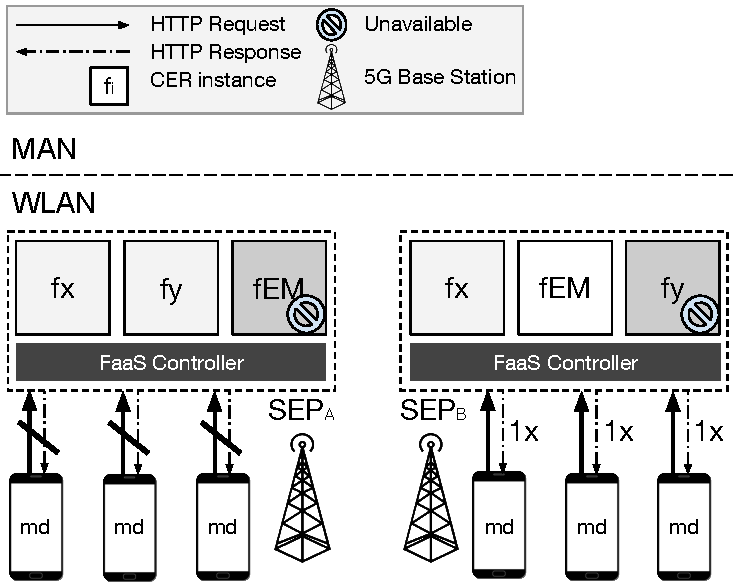
\includegraphics[width=0.47\textwidth]{Figs/Mobile_Computation_Offloading_F1.pdf}}
	~
	\captionsetup[subfigure]{width=0.515\linewidth}
	\subfloat[Data-intensive \textit{feature extraction} (fE) is performed by SEPs A and B; whereas \textit{feature matching} (fM) is offloaded from SEP A to B or a Regional SEP by a \textit{FaaS Controller}. In total, computation is offloaded with two (2x) \textit{HTTP requests} per video frame (SEP B), plus one (1x) inter-platform fM request (SEP A).\label{fig:Mobile_Computation_Offloading_F2}] {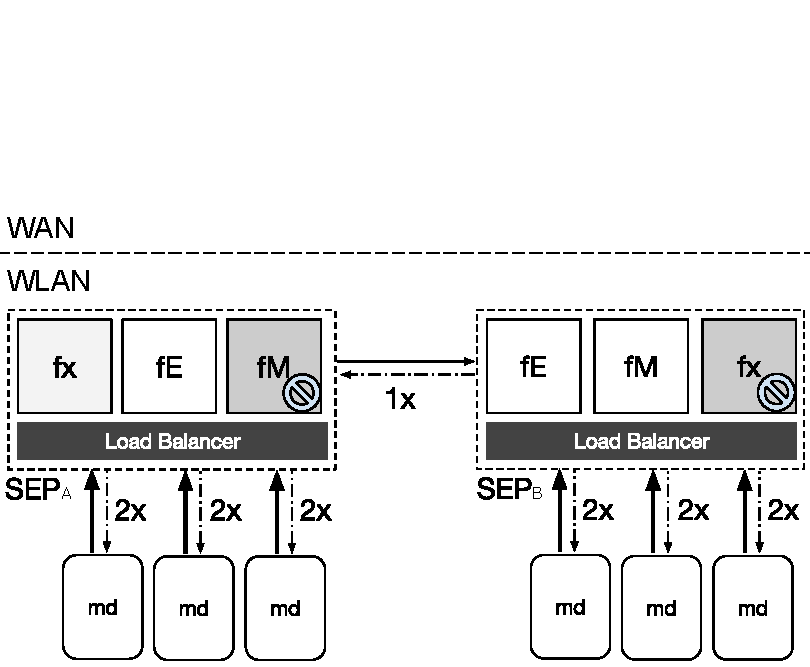
\includegraphics[width=0.515\textwidth]{Figs/Mobile_Computation_Offloading_F2.pdf}}
	\caption{\textit{Feature extraction} and \textit{matching} functions from the AR example forming a single (a), and two fine-grained services (b)} \label{fig:Mobile_Computation_Offloading}
\end{figure*}

Serverless computing~\cite{Lloyd18serverless,Roberts:2018} is mainly associated with two concepts: of applications that rely on third-party cloud services for handling business logic and state (also known as background-as-a-service, or BaaS); and that of applications for which server-side logic is still written by application developers, but, unlike traditional architectures, runs in stateless compute containers that are event-triggered
%, ephemeral (may only last for one invocation), 
and fully managed by a third party (also known as functions-as-a-service, or FaaS).

In the FaaS model, application logic is implemented as functions, which may be written in various languages and exposed as web services. Functions are packed along with dependencies (e.g., modules, libraries, and other resources); runtime instances (e.g., NodeJS, Python) are made available on demand within milliseconds, thanks to the container technology. Functions can be executed just once, frequently, or concurrently. After completion, containerized runtime instances may remain idle (warm) for a short period of time before been reused or released.

If compared to the conventional \textit{Infrastructure-a-as-Service} model (IaaS), the FaaS model ensures resources to be allocated when actually needed. FaaS platforms (e.g., AWS Lambda~\cite{AWSLambda}) also enforce limitations to the function package size and execution time by design. Due to its characteristics, this execution model enables an efficient usage of shared computational resources, which is particularly important to cope with the resource limitations of edge platforms and to allow edge-based solutions to scale~\cite{GarrigaMendonca2017}.



%The achieve efficiency is particularly important in the context of fine-grained edge nodes exhibiting limited computational and storage resources. 

%a higher number of concurring functions~\cite{}.

%

%Also, users are billed by the actual usage of resources (pay-as-you-go). This model may give edge infrastructure providers a .

%\subsection{Edge Infrastructure and Architecture}

%Regardless of...
\section{The Serverless Edge Platform}\label{sec:SEP}

\subsection{Mobile Computation Offloading}\label{sec:SEP_MCO}

The offloading of computation from mobile devices to cloud servers was firstly addressed by the concept of Mobile Cloud Computing~\cite{Khan:14}. Its main purpose was to enable rich mobile applications to be executed in resource-constrained mobile devices. However, this approach is limited by network latency, which is prohibitive for most real-time and interactive applications.

Addressing the network latency problem, \textit{cloudlets}~\cite{Satyanarayanan:2009} --- a precursor of edge computing --- have been proposed as resource-rich computer or cluster of computers  accessible through wireless local area network (WLAN). Their purpose is to enable the offloading of latency-sensitive computation from mobile and, more recently, general IoT devices. 

%To address this kind of edge computing scenario, an edge platform should support the execution of \textit{latency-sensitive} tasks. With the evolution of mobile devices capabilities, \textit{computing-intensive} tasks from real-time applications are of particular interest.

To illustrate this scenario, let us consider an Augemented Reality (AR) application that relies on two tasks: one for \textit{feature extraction} and another for \textit{feature matching}. The first handles the extraction of features from captured video frames, whilst the second matches theses features against a catalog (e.g., points of interest in a city area). 
%By offloading these tasks to a surrogate edge platform, the application is able to recognize more POIs while avoiding to stress the mobile device.
These computation-intensive, latency-sensitive tasks are strong candidates for been offloaded from hosting devices.

Targeting these requirements, a serverless edge platform (SEP) can exploit the FaaS model to allow tasks such as the \textit{feature extraction} and \textit{matching} to be written as stateless functions and consumed as web services. The resulting architecture would consist of two independent, fine-grained and highly cohesive FaaS-based services\footnote{We do not use the microservice terminology despite the characteristics of that FaaS-based services share with microservices}. Alternatively, both functions could compose a single, coarser service. Its main advantage would be the reduced communication overhead. However, in the context of edge computing, separating functions into distinct services has the following benefits: i) it allows different functions to be consumed independently by distinct applications (e.g., a common feature extracting service); and ii) it allows functions to be deployed and scaled independently.%; and iii) it allows the dynamic placement of functions into different edge and cloud platforms.

The last advantage is particularly important, as different types of edge infrastructures~\cite{Satyanarayanan:2009,Taleb:2013,Liu:2014,K.Wang:2015} converge in one aspect: their limitation of computational resources. The separation of functions with different responsibilities and requirements into independent services allows each function to be provided by distinct edge platforms; the decision of where to execute each function will depend on factors such as the characteristics and requirements of each function, the capabilities of distinct edge platforms, and the network latency and throughput among edge platforms and client devices. In a hierarchical topology~\cite{Liu:2014}, data-intensive functions are best candidates for been placed in close proximity to the edge, whereas computing-intensive functions may require more powerful resources from intermediary edge nodes. 

Figure~\ref{fig:Mobile_Computation_Offloading_F1} depicts the two AR functions as a single service (one request per offloading), whilst Figure~\ref{fig:Mobile_Computation_Offloading_F2} depicts each function as an independent service (two requests per offloading). 
In the first approach, mobile devices (md) connected to SEP A are unable to offload computation, as the fEM function is currently unavailable at that platform and the network throughput among these SEPs is insufficient for delegating requests with a video frame payload.
In the second approach, data-intensive \textit{feature extraction} (fE) is performed by both SEPs. Conversely, \textit{feature matching} (fM) is unavailable at SEP A; fM requests targeting this platform are offloaded to SEP B by its \textit{Load Balancer},
%or to the cloud by a load balancer, 
thanks to the reduced payload size (frame features extracted by fE) and the low latency among these surrogate platforms. 



%First, the FaaS model is based on events; 

\begin{figure}[tbp]
	\centering
	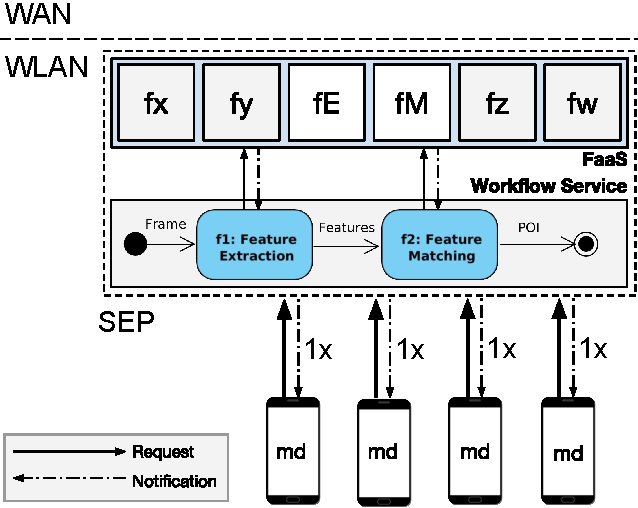
\includegraphics[width=\linewidth]{Figs/Mobile_Computation_Offloading_Workflow.pdf}
	\caption{An AR workflow involving the sequential execution of the \textit{feature extraction} (fE) and \textit{feature matching} (fM) functions; each video frame generates a single (1x) request, which is processed by one instance of each function.} 
	\label{fig:Mobile_Computation_Offloading_Workflow}
\end{figure}

Notwithstanding the benefits of the FaaS model, the satisfaction of low-latency requirements by the serverless edge platform requires further optimization.

%In the FaaS model
First, functions are externally triggered by HTTP requests. In the context of real-time applications, communication overhead must be kept minimal. As such, the edge platform must include an interface that allows clients to trigger sequential or parallel execution of functions composing different services without the overhead associated to the HTTP protocol. In this regard, the \textit{WebSocket protocol}~\footnote{https://tools.ietf.org/html/rfc6455}
%is a standardized protocol that 
provides full-duplex communication channels over a single TCP connection. %Figure~\ref illustrates this feature.

%For this, each task is deployed as a stateless, fully-managed function and exposed as a web service. 
%Within milliseconds, the fully-managed platform allocates a containerized runtime instance in which the function is first executed, whereas subsequent executions may take advantage of existing instances.
%Dependencies, if any, are described within a package descriptor and made available by the platform.
%Finally, a third function gets detailed information about each POI from a remote database.
%In particular, OpenWhisk is an state-of-art and open source FaaS platform.

The support for websockets would enable real-time interactions between mobile clients and the edge platform. Still, individual function invocations may add significant latency overhead whenever two or more functions form an execution flow. To avoid this overhead, developers would be forced to either chain function calls through hardcoded dependencies, or write coarser and less cohesive functions. Moreover, the chaining of function also imposes a cost overhead, since calling functions are kept waiting.% for other function(s) to return. 

To address latency, design, cost, and resource efficiency concerns, the SEPs should support \textit{function workflows}. This kind of service would allow developers to define, through visual or textual programming, a function execution flow.
%starting with the processing of the input sent by a client and finishing with the result sent back to the client. 
Similarly to functions, workflows are triggered by events; at each intermediary step, result from one function is passed to the subsequent function call. Going back to the AR example, Figure~\ref{fig:Mobile_Computation_Offloading_Workflow} depicts a simple workflow consisting of the sequential execution of the \textit{feature extraction} and \textit{matching} functions, which remain decoupled.% of each other.

\begin{figure}[tbp]
	\centering
	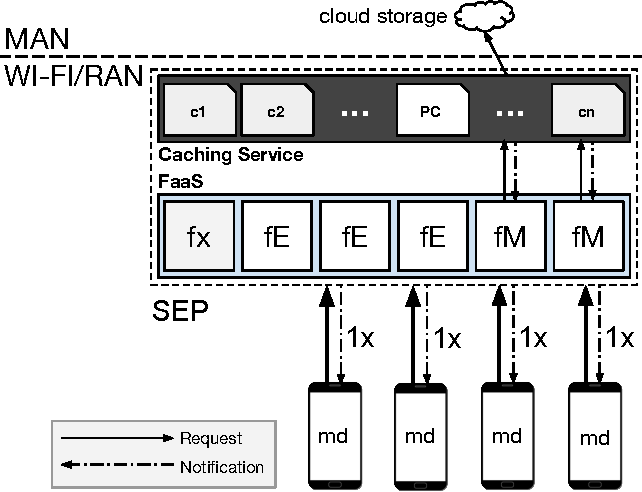
\includegraphics[width=\linewidth]{Figs/Mobile_Computation_Offloading_Caching.pdf}
	\caption{A SEP with three instances of the \textit{feature extraction} (fE) and two instances of the \textit{feature matching} (fM) functions; a local copy of the POI catalog (PC) is fetched once from a cloud storage service and served to the fM instances.} 
	\label{fig:Mobile_Computation_Offloading_Caching}
\end{figure}

Last but not least, existing FaaS platforms (e.g., AWS Lambda and Apache OpenWhisk) enforce a programming model in which functions have access to a transient folder without guaranteeing that subsequent invocations will be executed by the same containerized environment. %Thus, each invocation must check whether cached data is available. 
In the context of real-time applications, retrieving extensive data sets may add prohibitive overhead. For instance, in the AR example, a POI catalog (circa 1Gb) is employed to identify points of interest against their matched features. Due to size limitations, it can not be packed with the function source code, but needs to be retrieved dynamically.
%Cloud vendors provide storage services as part of their platform ecosystem. 

%To address the need of edge services with dependency to large data sets
Addressing the aforementioned issue, we propose to equip SEPs with a caching service. This service should fetch data from cloud-based storage services and keep it available locally for mitigating networking overhead. 
%More precisely, it consists of an object-based storage system, in which files are associated with metadata. 
To make use of this service, SEP functions request files passing their cloud URI, which should return a valid file format.
% --- and an optional expiration policy. 
Once retrieved, the caching service stores the file along with the metadata containing its URI and frequency of access; subsequent requests are served without networking overhead. 
Figure~\ref{fig:Mobile_Computation_Offloading_Caching} illustrates the interplay between the caching service storing a POI catalog (PC) retrieved from a cloud storage and multiple runtime instances of the \textit{feature matching} function.

%TODO: move this to the prototype section?
%To support different kinds of edge infrastructure, the SEP caching service should rotate cached files according to the availability of storage resources and the access frequency of cached files. As such, files accessed less frequently are subject for been replaced in case of resource contention. 
%%Files without an expiration date are replaced only in case of resource contention following the access frequency policy. 


%A serverless edge platform should support a more efficient caching service to optimize use cases in which functions have data dependencies. 
\subsection{Edge Data Analysis}

\begin{figure}[tbp]
	\centering
	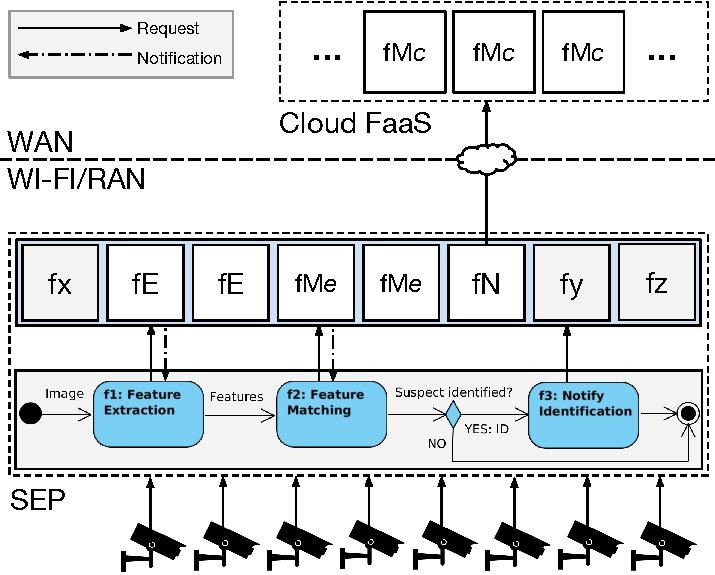
\includegraphics[width=\linewidth]{Figs/Edge_Data_Analytics_Video_Surveillance.pdf}
	\caption{Features from video frames captures by surveillance cameras are extracted (fE) and, upon a positive matching (fM$e$), sent for further analysis by a cloud service (fM$c$).}
	\label{fig:Edge_Data_Analytics_Video_Surveillance}
\end{figure}

More recently, the advent of data-intensive Internet of Things (IoT) devices and applications raised concerns about the feasibility of sending exponentially larger volumes of data through the Internet all the way to cloud data centres. Accordingly, another important motivation for edge computing consists of the anticipation of the analysis of data produced and consumed by applications at the network edge. 

%TODO: find an example with low-latency requirement?
%Differently from the mobile computation offloading scenario, the most important concerns of edge data analysis are network throughput 
%(to cope with large volumes of data) 
%and preventing network bottlenecks caused by centralization. Still, edge analysis may also need to cope with low-latency requirements, specially if analysis results should feed latency-sensitive actuation.

%To illustrate this scenario
For example, in the context of smart cities and cyber-physical-systems, let us consider a video surveillance application depicted by Figure~\ref{fig:Edge_Data_Analytics_Video_Surveillance}. Similarly to the AR application, compute-intensive functions such as \textit{feature extraction} (fE) and \textit{matching} (fM\textit{e}) are assigned to edge platforms.
%, this time with the purpose of recognizing faces from a police catalog. 
These functions compose a workflow exposed as a service and consumed by resource-constrained IoT cameras. This service receives video frames at short intervals, from which it extracts facial features matched against a police catalog (PC). A positive identification triggers the execution of a cloud-based service (fM\textit{c}) responsible for a more robust analysis able to detect false positives. In this manner, large volumes of data are processed at the edge, preventing the congestion of the wide area network (WAN) and the centralized services.

\begin{figure}[tbp]
	\centering
	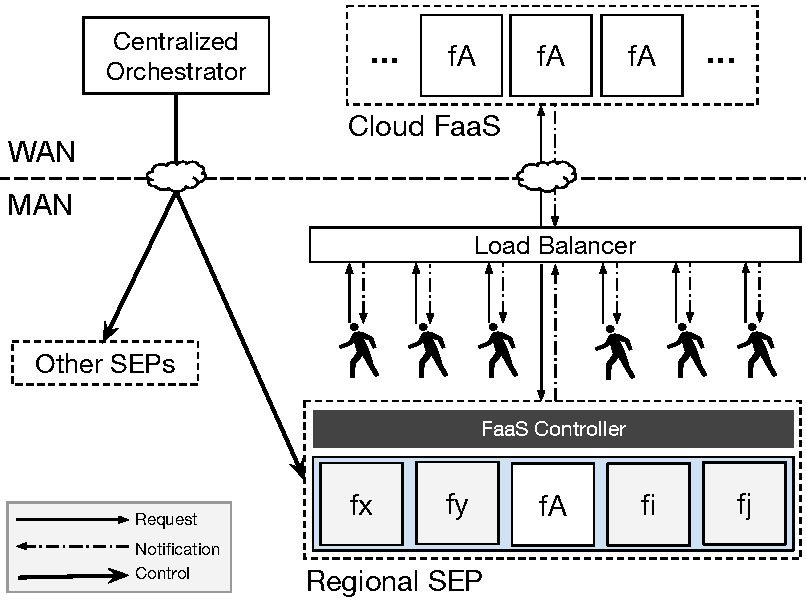
\includegraphics[width=\linewidth]{Figs/Edge_Data_Analytics_Personal_Assistant.pdf}
	\caption{Instances of the \textit{health analysis} function (fA) are placed to SEPs by a centralized \textit{Orchestrator}; given the current placement scheme, a \textit{Load Balancer} distributes requests among its local FaaS and the cloud-based FaaS based on the fA requirement for latency and the average response time.}
	\label{fig:Edge_Data_Analytics_Personal_Assistant}
\end{figure}

Still in the context of edge data analysis, 
%other use cases exhibit more strict requirements for latency. For instance, 
let us imagine that in the future the majority of elderly citizen will be wearing body sensors to collect data about their health status. In the event of an anomalous condition (e.g., the beginning of a heart attack), emergency services should be dispatched immediately to the person location. Moreover, it is very important to provide the person with feedback so she can ask nearby people for their assistance.
%other people that can provide a first and immediate assistance.
%The IoT-based heart disease monitoring system for pervasive healthcare service
The accurate identification of such events, however, requires complex analysis of data from different sensors (e.g., heart rate, oxigen saturation, glucose~\cite{Li:2017}). Offloading the analysis from all users to the cloud may overload the network and centralized services. Instead, this burden should be shared with SEPs.% composing the mobile networks infrastructure (e.g., base stations, multi-technology aggregation sites, etc~\cite{}). 

The aforementioned examples share one characteristic: their main purpose is to prevent large volumes of data to be sent and processed by distant data centres. In the latter example, providing feedback in a timely manner is important, but does not fall into the category of low ($\leq 100ms$) or ultra-low ($\leq 20ms$) latency requirements. For this kind of application, the offloading of data analysis from the cloud to the edge should be opportunistic and informed by the availability of computing and networking resources, as well as the latency requirement of each function.

As discussed in Section~\ref{sec:SEP_MCO}, the proposed architecture (see Figure~\ref{fig:Mobile_Computation_Offloading}) enables fine-grained functions to be placed onto different platforms. Differently from real-time computation offloading, it now includes cloud-based platforms. This decision can be either orchestrated by a centralized entity~\cite{Taleb:2013}, coordinated among different edge and cloud platforms~\cite{Mach:2017}, and involve the participation of client devices~\cite{Baresi:2018}. Based on a given placement scheme, an informed \textit{Load Balancer} makes the timely decision on the destination of each request arriving at its own SEP.

%Differently from the mobile computation offloading scenario, edge data analysis may tolerate higher delays, in which case a \textit{scheduler} should decide between edge-based and cloud-based services. 

%TODO: improve the scheduling explanation
Figure~\ref{fig:Edge_Data_Analytics_Personal_Assistant} presents the opportunistic placement of a \textit{health analysis} function (fA) onto edge and cloud platforms. Based on the availability of resources at the SEP and the demand for different services, a centralized \textit{Orchestrator} decides for the number of instances hosted by the SEP. In turn, the SEP \textit{Load Balancer} assigns incoming requests to its local FaaS or to the cloud-based FaaS, taking into account the latency requirement and the average response time. Upon a heath emergency, the function proceeds with two actions: i) the invocation of an emergency service; and ii) the notification of the personal assistant device about the emergency. For this, the \textit{Load Balancer} must also work as a \textit{reverse proxy} to assure results will be sent back to client devices regardless of the platform each request have been assigned to.

%In particular, the scheduling should take into account the latency constraints of each type of service.

%For instance, let us consider the case of a mobile crowd sensing application in which environmental data (e.g., air pollution~\footnote{a common type of sensor in smartphones in China}) is collected from sensors embedded in smartphones, tablets, and variables accompanying people. 

%This example poses one challenge: if functions are stateless and their instances ephemeral, how should the platform deal with long-living cases of data analysis? 

\subsection{Stateful Edge Services}

\begin{figure}[tbp]
	\centering
	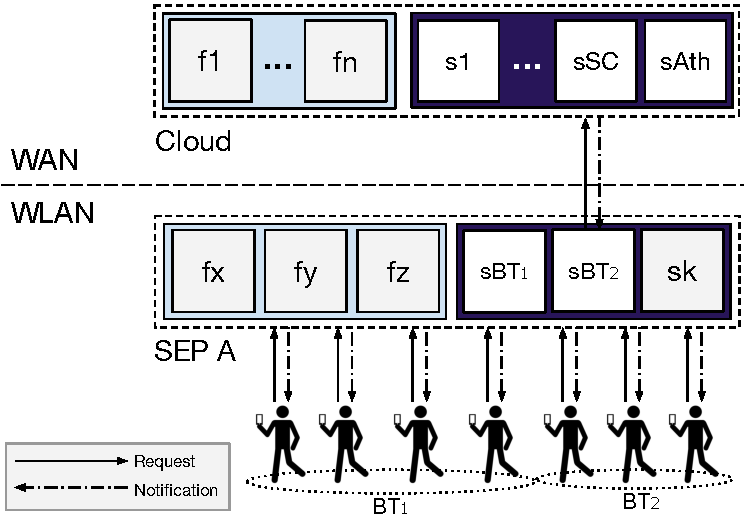
\includegraphics[width=\linewidth]{Figs/Stateful_Edge_Services.pdf}
	\caption{A stateful service enables multiple players to join game battle sessions (BT$_1$, BT$_2$); instances (sBT$_1$, sBT$_2$) are mapped to each session; authentication (sAuth) and player scores (sSC) are managed by cloud-based services.}
	\label{fig:Steteful_Edge_MMG}
\end{figure}

One of the most important directives concerning the design of web services is to move state into a separate layer~\cite{Armbrust:2010}. Stateless services are easier to test, debug, and scale, whereas stateful services require state to be recreated for testing and debug purposes, and achieving consistency among replicated instances incur in performance degradation. However, some application scenarios exhibit particular needs that justify the adoption of stateful services.


To illustrate this requirement, let us think of a mobile multiplayer game (MMG). As an interactive application, low-latency is a first class requirement that justifies the deployment of services to the network edge. As an example, \textit{PokemonGO}, a popular MMG, features a single interactive use case in which players interact with virtual \textit{Pokemons}~\footnote{A fantasy creature collected by players} added to their devices screen. 
%

To increase the game popularity, a new interactive feature could enable users in the same city area to start game battles involving their \textit{Pokemons}. Following a conventional multiplayer game architecture, an authoritative service is designed to host the game battle state and business logic. In particular, the state represents a battle session, whilst business logic is responsible for updating the state according to user inputs and other events. 

Addressing the aforementioned example, the solution depicted in Figure~\ref{fig:Steteful_Edge_MMG} exploits two benefits from stateful services: first, it prevents the overhead of transferring to the service, at each user interaction, the whole state of the battle; second, it allows an authoritative service to manage changes to the game state that may not be safely delegated to clients, who otherwise could modify the local game logic and state to their own advantage.
%(e.g., in a P2P architecture)
Composing the rest of the application, other delay-tolerant features (e.g., players scores) should be managed by resourceful, long-living cloud-based services, accessed without SEP inter-mediation. Finally, to prevent the overhead associated with replicated state, stateful instances should be vertically scaled --- with the dynamic allocation of CPU/memory resources --- in detriment of horizontal scaling through instance replication. %Figure~\ref{fig:Steteful_Edge_MMG} depicts the resulting architecture.%; instances of the stateful \textit{multiplayer battle service} are hosted by the serverless edge platform precisely when needed. 

The support for stateful services comes with a cost. To address the specific use cases requiring stateful services, a serverless edge platform should impose limitations. More precisely, stateful services should be designed to last for a limited duration corresponding to the lifetime of a specific latency-sensitive use case. Similarly to its stateless counterpart, it should be created and terminated on demand in a timely manner without preallocating resources.

\subsection{Real-time Edge Coordination}

Another important application scenario involves the real-time coordination among distributed mobile and IoT devices at the network edge. To illustrate this scenario, let us consider the coordination among Autonomous Vehicles (AV). Each vehicle is expected to generate large volumes of data from its sensors, including the AV's actual position, speed, and acceleration. AVs make use of sophisticate mechanisms to prevent collisions. Notwithstanding this, AVs traveling at high speeds would benefit from real-time notifications of anomalous events in their path (e.g., accidents). 

To address real-time coordination among edge devices, SEPs can feature a publish-subscribe (pub-sub) notification service. This service would allow edge devices (e.g., AVs, surveillance cameras) to coordinate with other devices and additional systems integrated with the edge platform (e.g., a road monitoring system). In addition to localized coordination, surrogate SEPs must form a distributed event bus, enabling inter-platform coordination (e.g., AVs and cameras connected to different SEPs). Other edge-based systems (e.g., an emergency service) could also subscribe to anomalous events in order to take actions (e.g., to dispatch ambulances or road patrols) in a timely manner.

The integration enabled by a pub-sub service fits well in a serverless architecture~\cite{Lloyd18serverless}. Indeed, existing FaaS platforms (e.g., AWS Lambda~\cite{AWSLambda}) are integrated with other systems by means of notification services (e.g., AWS SNS) in which functions are triggered by event notifications. In the AV coordination example, a similar approach could be used to trigger, upon an anomalous event, a specific function responsible for the invocation of an external service (e.g., a cloud-based service that persists the occurrence of the anomalous event). 

\begin{figure}[tbp]
	\centering
	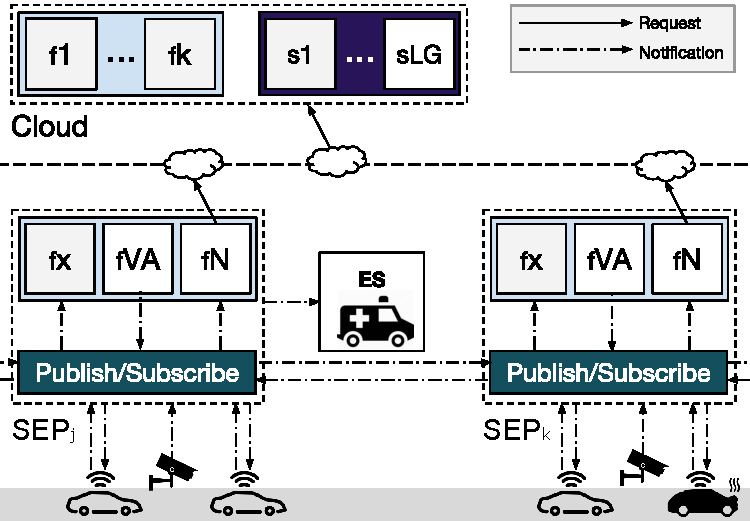
\includegraphics[width=1\linewidth]{Figs/Edge_Coordination_AVs_wide.pdf}
	\caption{Autonomous Vehicles, a road monitoring system, an emergency service and a logging service are coordinated by means of a distributed event bus hosted by surrogated SEPS}
	\label{fig:Edge_Coordination_AVs}
\end{figure}


Figure~\ref{fig:Edge_Coordination_AVs} illustrates the solution for the AVs coordination example. AVs subscribe to the pub-sub service hosted by surrogate SEPs; anomalous events --- reported by AVs or video analysis functions (fE and fM) --- are propagated to the AVs within its own SEP zone, to those behind, and to an emergency service (ES). Finally, a cloud-based logging service (sLG) is invoked by a SEP-based notification function (fN). In order to prevent multiple invocations of the logging service, the notification function at each SEP must distinguish between local events and those from other platforms. The same is valid for the emergency squad service covering different road sections. To satisfy this requirement, the pub-sub service should enforce location-awareness by mapping each event to its SEP of origin.

%\subsection{On Premise Edge}

%Serverless computing has been conceived as a cloud model. Notwithstanding this, a serverless architecture can be adopted by on premise edge infrastructure to deliver self-managed services to smart home, office, and Industry 4.0 applications. For this, on premise SEPs should exhibit the computational resources and services (discussed along the present section) compatible with targeted applications. 

%Also, on premise and on demand SEPs can form an infrastructure continuum supporting mobility.

%We conclude the present section with a typical smart home scenario in which a plethora of sensors providehttps://www.overleaf.com/project/5bb1f5b57d8ebf292d2436ed information about the environment and actuators operate on different equipment. Communication with the domestic SEP is performed with lightweight protocols (e.g., COAP~\cite{} and MQTT~\cite{}). Functions are triggered by events (e.g., from sensors), direct calls (e.g., from smart devices) or execution flows (e.g., from a microclimate analysis workflow). Figure~\ref{} illustartes this scenario.

\section{SEP Prototype}~\label{sec:prototype}

With the purpose of demonstrating the feasibility of the proposed platform, we assembled state-of-art tools materializing the architecture and services discussed throughout Section~\ref{sec:SEP}. We also propose extensions to the architecture and implementation of \textit{OpenWhisk}, an open source FaaS platform.

%, evaluating it in different aspects. 
%Figure~\ref{fig:Serverless_Edge_Platform_Overview} presets an overview of the SEP prototype containing all the proposed services. In addition to the services discussed in Section~\ref{sec:SEP}, it includes a \textit{Reverse Proxy}, which is responsible for proxying external HTTP/WebSocket requests to internal platform services.

\subsection{OpenWhisk}

OpenWhisk~\cite{OpenWhisk} is a state-of-art tool implementing the FaaS model. Originally developed by IBM, it is now an open source project incubated by Apache. It is also the most mature open source FaaS tool available. 

OpenWhisk plays a central role in the proposed SEP architecture %First and foremost,
%as it takes care of the dynamic creation and termination of containerized environments. More precisely, 
by handling the creation and termination of \textit{Docker} containers
%\footnote{Other less popular container engines are also supported} 
with a specific runtime supporting the execution of stateless functions. Functions are activated by rules associated with triggers, which in turn are mapped to internal and external events, including HTTP(S) requests. %TODO: activations, syncrhonous and asynchronous requests

OpenWhisk features a service-oriented architecture.
Among others, it comprises the following components~\cite{OpenWhisk}:

\begin{itemize}

    \item \textit{Nginx}: a multi-purpose tool featuring a \textit{reverse proxy}; this component enables the external invocation of the platform \textit{API}, including the upload and triggering of \textit{functions};
    
    \item \textit{Controller}: responsible for validating, authenticating, and distributing (load balancing) requests to \textit{Invokers}; and 
    
    \item \textit{Invoker}: responsible for the management of a pool of CERs, including their creation upon function activation and termination upon idleness;
    
    
    %selecting or creating a CER for the execution of a function activation.
    
\end{itemize}

\begin{figure}[tbp]
	\centering
	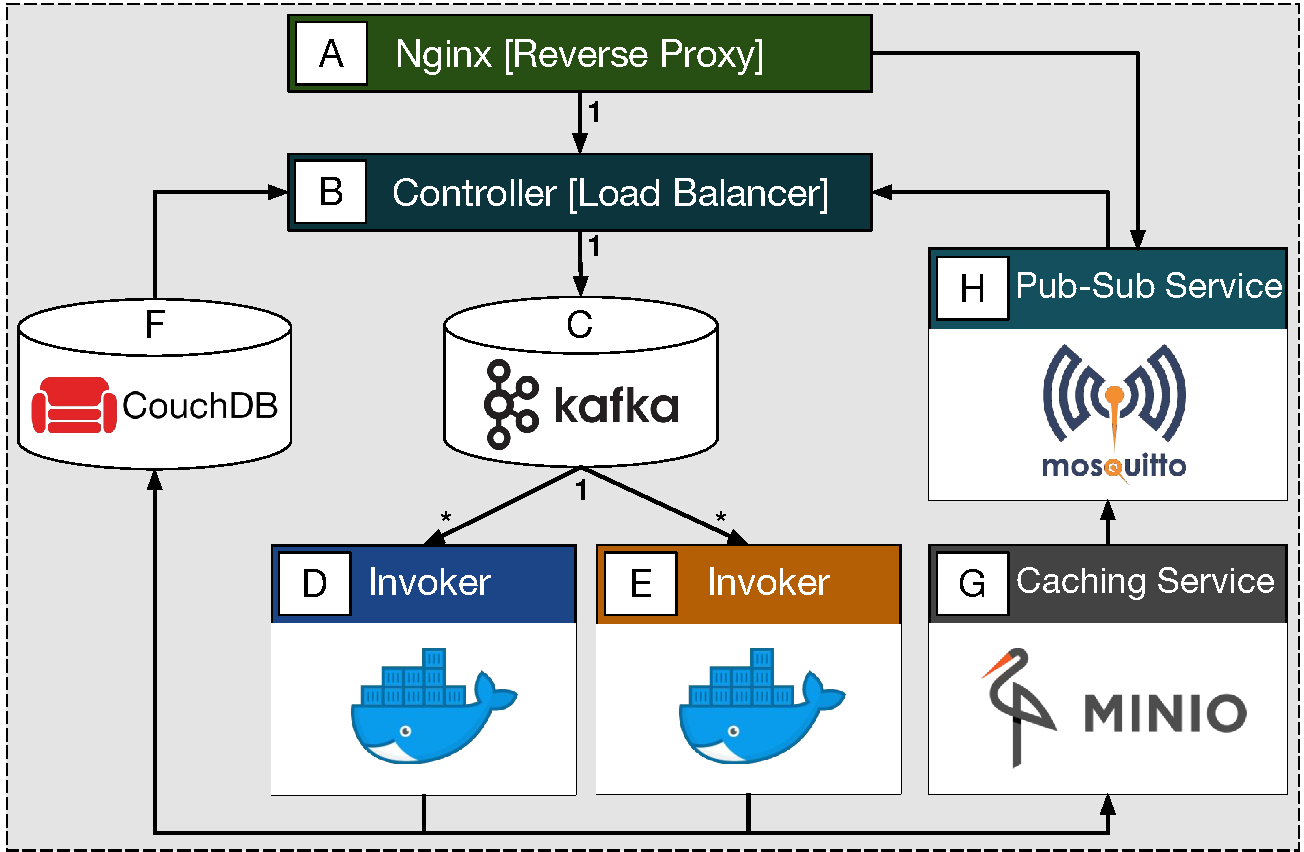
\includegraphics[width=1\linewidth]{Figs/Serverless_Edge_Platform_Prototype.pdf}
	\caption{Overview of the SEP prototype comprising all tools and services}
	\label{fig:Serverless_Edge_Platform_Overview}
\end{figure}

\subsection{Latency-Sensitive Computation Offloading}

%TODO ETSI comparison
To cope with the requirements of latency-sensitive computation offloading, SEP components are deployed to fog nodes in close proximity with end-users (e.g., cloudlets and cellular infrastructure). In this configuration, client devices interface with  OpenWhisk's \textit{Controller} through its \textit{Reverse Proxy} (Nginx).

%the critical path that starts with the client request and finishes with the response notification must remain near the edge. 


Depending on the installed capabilities, OpenWhisk's \textit{Invoker} can be deployed to one or multiple VMs. Each \textit{Invoker} takes care of a pool of containers whose maximum size depends on the available resources. The load is distributed among \textit{invokers} by OpenWhisk's \textit{Load Balancer}.
%, who monitors the health status of each \textit{Invoker}.

OpenWhisk's \textit{Invoker} adopts a pure event-driven approach. Upon a function invocation, the \textit{Invoker} checks for the availability of a warm (idle) CER before creating a new one. To mitigate cold start of latency-sensitive functions, the \textit{idleness time} has been increased from \textit{50 milliseconds} to \textit{5 seconds}. More robust extensions targetting a more efficient resource allocation should consider a dynamic and autonomous optimization of this parameter.

OpenWhisk does not provide native support for the \textit{WebSocket} protocol. Coherently with what has been discussed in Section~\ref{sec:SEP_MCO}, we have extended OpenWhisk to enable a more efficient communication between SEPs and edge devices hosting real-time and interactive applications. The proposed extension consists of the following modifications: 

\begin{itemize}
    
    \item a new endpoint entry supporting the \textit{WebSocket} protocol in \textit{Nginx}'s configuration; and
    
    \item the additional implementation handling \textit{WebSocket} messages in the \textit{Controller} component.
    
\end{itemize}

%upon the activation of actions --- a stateless function written in one of the many languages supported by the tool.
%OpenWhisk is implemented as an event-driven platform. 

OpenWhisk natively supports action sequences, which allow the creation and triggering of sequential execution flows using the platform's API. Our prototype exploits this feature for the definition of the \textit{Workflow Service} discussed in Section~\ref{sec:SEP_MCO}. Future extensions may consider the support of more comprehensive flow-based languages. %(e.g., from visual programming tools such as \textit{NodeRED}).


%\subsection{Caching Service}

Finally, for the materialization of the \textit{Caching Service} discussed in Section~\ref{sec:SEP_MCO}, we adopted \textit{Minio}, an open source and lightweight object storage tool already part of OpenWhisk stack.
Minio is compatible with \textit{AWS S3} --- a state-of-art object storage service --- and features native integration with different types of notification systems. Moreover, it features an API for managing objects. These characteristics are particularly important in the context of a SEP platform, as object events (e.g., creation, update) can trigger the execution of functions, whereas functions have access to objects through API calls. 

%an event-driven serverless architecture

%a prototype of the caching service discussed in ~\ref{sec:SEP_MCO} was implemented as a separated module in Python language. Figure~\ref{fig:SEP_Low_Latency_FaaS} presents the resulting platform architecture.

%existing containers and an \textit{Invoker} responsible for the creation and termination of containers. 


\subsection{Opportunistic Edge Data Analysis}

OpenWhisk lacks support for the dynamic placement of functions based on latency requirements and other criteria. Nonetheless, it features a \textit{Load Balancer} that decides, among distributed \textit{invokers}, where to send requests. 
%Each pool is interfaced and managed by an \textit{Invoker} component. 
The \textit{Load Balancer} communicates with OpenWhisk's \textit{Invoker} through messages buffered and persisted by \textit{Apache Kafka}, a high-throughput, distributed, publish-subscribe messaging system.
%(see Figure~\ref{fig:Serverless_Edge_Platform_Overview}). 

%an implementation of the \textit{Actor Model} featuring reliable queues.

To evaluate the feasibility of the opportunistic placement discussed in Section~\ref{sec:SEP_EDA}, our prototype configures OpenWhisk to be aware of two invokers: a local one mimicking an edge deployment, and another hosted by a remote node mimicking a cloud deployment. It required two interventions: 

\begin{itemize}
    \item the initialization of an external (cloud) \textit{Invoker} referencing the SEP \textit{Load Balancer}'s public IP; and
    
    \item the prioritization by the \textit{Load Balancer} of the local \textit{Invoker} whenever the response time is below a threshold. %the CPU or memory load at the SEP is below 90\%. 
\end{itemize}

The opportunistic placement prototype also required modifications from the \textit{Invoker} side. More precisely, function activation now takes as parameter the \textit{maximum number of CER instances} each function can have --- as decided by an \textit{Orchestrator}. If this limited is achieved, the function activation fails and the original request is put back into the \textit{Load Balancer} queue. As the response time increases above the threshold, requests are diverged by the \textit{Load Balancer} to the cloud platform. 

Finally, an \textit{Orchestrator} was implemented as a separated module in Python language. Its simple role is to monitor the arrival rate of different functions and inform the SEP for the share of resources each function may allocate.


%Figure~\ref{fig:SEP_Low_Latency_FaaS} presents the resulting platform architecture.

%TODO
Figure~\ref{fig:SEP_Placement} presents the resulting architecture with the \textit{Load Balancer} part of the \textit{Controller}. While this configuration is suitable to SEPs in close proximity with end-users (e.g., co-located with WLAN or RAN infrastructures), it may add substantial latency if the SEP lies many network hops away from the natural path to the cloud alternative. In this case, external \textit{load balancers} should anticipate request distribution among local, regional, and cloud-based SEPs (see Figure~\ref{fig:Edge_Load_Placement}).

%or become a bottleneck in intermediary deployments (e.g., regional SEPs covering larger areas). 


%The evaluation of more sophisticated orchestration strategies is out of the scope of this work. 

%Contrasting with real-time FaaS, we further extended OpenWhisk's Load Balancer with scheduling capabilities. The idea is to take different latency requirements into account and prioritize those with more strict deadlines. For this, requests arriving at the SEP's Controller are sorted by means of a \textit{deadline first} algorithm before been distributed by the Load Balancer.

\subsection{Stateful Services}

To address the need of stateful services, we have enabled stateful application partitions to run in a similar environment from stateless functions by extending OpenWhisk's \textit{Invoker}. In contrast with stateless functions --- which can be executed by any available or new CER with the corresponding runtime --- stateful services are identified by a token mapped to one specific CER upon initialization (\textit{session start event}). 

Every invocation to the stateful service is delegated to the corresponding CER by means of an \textit{update command}. This additional command specifies the service function to be performed along with any parameters from the original request. The resulting mechanism enables state to be consistently evolved at each invocation from one or distinct clients within the same session until CER termination (\textit{session end event}).

%Figure~\ref{} illustrates the stateful service life-cycle.

\subsection{Real-time Edge Coordination}

%Among the stack of technology composing OpenWhisk lies \textit{Kafka}, a high-throughput, distributed, publish-subscribe messaging system. 

The need for a publish-subscribe notification service is addressed with the adoption of \textit{Mosquitto}, an open source MQTT implementation largely adopted by IoT practitioners. %MQTT is the standard protocol for IoT machine-to-machine communication. 
Among its features, its \textit{broker} enables \textit{topic bridging} and \textit{remapping}. The former allows two or more brokers to become publish/subscribers of each other, so that messages published to one broker are propagated. In turn, topic renaming allows the definition of prefixes to the topics propagated from/to other brokers. The platform prototype exploit these features to allow the propagation of events from/to surrogate SEPs, as discussed in Section~\ref{sec:SEP_RTEC}. %Figure~\ref{} illustrates the resulting architecture.

\subsection{Nginx}\label{sec:prototype_Nginx}

Last but not least, SEPs should interface with the external world by means of a reverse proxy. Its role is to map external requests (e.g., HTTP, WebSocket) to internal services (e.g., FaaS, publish-subscribe system, etc). 

Nginx is a state-of-art tool open source tool featuring, among others, a reverse proxy. Similarly to Apache, it allows the specification of endpoints that are mapped to internal applications. Due to its maturity and popularity, we adopted Nginx as the reverse proxy in our SEP prototype. This tool is also naively integrated with OpenWhisk.

%\subsection{SEP Product Line}

%TODO: contextualize the paragraph below
%Figure~\ref{} represents the serverless edge platform as a software product line~\cite{} with product variants targeting different types of edge infrastructure and application scenarios.

\section{Evaluation}\label{sec:evaluation}
\section{Conclusions and Future Work}\label{sec:conclusions}

In this work we tackled the materialization of a platform for edge and fog computing with a serverless architecture. Different applications scenarios were matched with platform services; we also presented the rationale for inter-platform cooperation and management. A prototype extending a state-of-art FaaS platform was evaluated in terms of memory footprint, latency, throughput, and scalability. Obtained results corroborate the benefits of the serverless architecture and the feasibility of the proposed \textit{Serverless Edge Platform} in fulfilling the requirements from different types of application scenarios in heterogeneous fog node deployments. 

As future work, we are particularly interested in deepening 
two aspects: i) the decentralized inter-platform cooperation through delegation of requests to surrogate SEPs; and ii) the opportunistic placement of functions onto SEPs in a N-tier fog deployment through hierarchical orchestration to enable the co-existence of both latency-sensitive computation offloading and edge data analysis scenarios. Finally, we also envision the evaluation of the proposed platform services targeting larger scale deployments such as regional SEPs.


% conference papers do not normally have an appendix

% use section* for acknowledgment
\section*{Acknowledgment}

The authors would like to thank...



% trigger a \newpage just before the given reference
% number - used to balance the columns on the last page
% adjust value as needed - may need to be readjusted if
% the document is modified later
%\IEEEtriggeratref{8}
% The "triggered" command can be changed if desired:
%\IEEEtriggercmd{\enlargethispage{-5in}}

% references section

% can use a bibliography generated by BibTeX as a .bbl file
% BibTeX documentation can be easily obtained at:
% http://mirror.ctan.org/biblio/bibtex/contrib/doc/
% The IEEEtran BibTeX style support page is at:
% http://www.michaelshell.org/tex/ieeetran/bibtex/
\bibliographystyle{IEEEtran}
% argument is your BibTeX string definitions and bibliography database(s)
\bibliography{bibliography}
%
% <OR> manually copy in the resultant .bbl file
% set second argument of \begin to the number of references
% (used to reserve space for the reference number labels box)
%\begin{thebibliography}{1}

%\bibitem{IEEEhowto:kopka}
%H.~Kopka and P.~W. Daly, \emph{A Guide to \LaTeX}, 3rd~ed.\hskip 1em plus
%  0.5em minus 0.4em\relax Harlow, England: Addison-Wesley, 1999.
%\end{thebibliography}




% that's all folks
\end{document}


